\documentclass[10pt]{article}
% AMS packages for better math typesetting
\usepackage{amsmath,amssymb,amsthm}
% To control the margin sizes
\usepackage{setspace}
% more options with enums and item lists
\usepackage{enumitem}

% For Finite Automata
% See: http://tex.stackexchange.com/a/20786/9247
\usepackage{tikz}
\usetikzlibrary{automata,positioning}


% Setting more standard margins
\setlength{\textheight}{9in} \setlength{\topmargin}{-.5in}
\setlength{\textwidth}{6.5in} \setlength{\oddsidemargin}{0in}
\setlength{\evensidemargin}{0in}

% Setup Math Forms
% See: http://web.mat.bham.ac.uk/R.W.Kaye/latex/thm.pdf
\newtheorem{theorem}{Theorem}
\newtheorem{lemmma}{Lemma}

\theoremstyle{definition}
\newtheorem{dfn}{Definition}


\title{ Simplifying NFAs \\ \small{Proof Paper Example} }
\author{James Logan Mayfield}


\begin{document}
\maketitle

\section{ Problem }

In this paper we consider the problem of converting an NFA with more than one accept state to an equivalent NFA with a single accept state.  For example, consider the NFA shown in Figure~\ref{nfa1}.

\begin{figure}[htbp!]
  \begin{center}
  \begin{tikzpicture}[shorten >=1pt,node distance=2cm,on grid,auto]
    \node[state,initial](q_0){$q_0$};
    \node[state](q_1)[right=of q_0]{$q_1$};
    \node[state,accepting](q_2)[below=of q_1]{$q_2$};
    \node[state](q_3)[above=of q_1]{$q_3$};
    \node[state,accepting](q_4)[right=of q_3]{$q_4$};
    \path[->]
    (q_0) edge node {b} (q_1)
          edge [swap] node {c} (q_2)
          edge node {a} (q_3)
    (q_1) edge [loop right] node {a,b,c} ()
    (q_2) edge [loop below] node {a,b} ()
          edge [swap] node {c} (q_1)
    (q_3) edge node {a,b} (q_1)
          edge node {c} (q_4)
    (q_4) edge [loop above] node {a,b,c} ();
  \end{tikzpicture}
\end{center}
\caption{An NFA with Many Accept states}
\label{nfa1}
\end{figure}

We might wish to unify the two accept states in this NFA in order to have a simpler machine with a single accept state and single starting state. The NFA shown in Figure~\ref{nfa2} is such a machine and accepts the same language as that of the machine in Figure~\ref{nfa1}. The new machine makes use of $\varepsilon$ transitions to move from old accept states to a new accept state.

\begin{figure}[htbp!]
  \begin{center}
  \begin{tikzpicture}[shorten >=1pt,node distance=2cm,on grid,auto]
    \node[state,initial](q_0){$q_0$};
    \node[state](q_1)[right=of q_0]{$q_1$};
    \node[state](q_2)[below=of q_1]{$q_2$};
    \node[state](q_3)[above=of q_1]{$q_3$};
    \node[state](q_4)[right=of q_3]{$q_4$};
    \node[state,accepting](q_5) [right=of q_2]{$q_5$};
    \path[->]
    (q_0) edge node {b} (q_1)
          edge [swap] node {c} (q_2)
          edge node {a} (q_3)
    (q_1) edge [loop right] node {a,b,c} ()
    (q_2) edge [loop below] node {a,b} ()
          edge [swap] node {c} (q_1)
          edge [swap] node {$\varepsilon$} (q_5)
    (q_3) edge node {a,b} (q_1)
          edge node {c} (q_4)
    (q_4) edge [loop above] node {a,b,c} ()
          edge node {$\varepsilon$} (q_5);
  \end{tikzpicture}
\end{center}
\caption{A Single Accept state version of the NFA shown in Figure~\ref{nfa1}}
\label{nfa2}
\end{figure}

The process used to generate the NFA shown in Figure~\ref{nfa2} can be generalized for any NFA\@ and this generalization leads to the following theorem.

\begin{theorem}
For any NFA $N$ with more than one accept state there exists an equivalent NFA $N^\prime$ with only one accept state.
\label{th}
\end{theorem}

We now prove Theorem~\ref{th} by providing a general process for construction $N^\prime$ and proving the equivalence of the language of $N$ and $N\prime$.

\section{ Proof Sketch }

In this paper we prove Theorem~(\ref{th}) by giving a construction for an equivalent NFA with a single accept state. The crux of the construction is the addition of $\varepsilon$ transitions from the original accept states to a new, singular accept state. Any string in the language of the original machine will terminate in an old accept state. The new accept state is then reached by taking the $\varepsilon$ transition to the new accept state. Strings not in the language that find themselves in the new accept state can be rejected by adding a transition out of the accept state to a garbage state that must be taken for any letter of the alphabet or by leaving transitions out of the new accept state undefined and thereby implying the rejection of any non-empty string in the accept state.

\section{ Proof }

The proof of Theorem~\ref{th} takes place in two parts. The first part is a procedure for constructing a NFA with a single accept state given an arbitrary NFA $N$\@. The construction is done in terms of the formal definition of a NFA and basic set theory. It requires no deeper consideration. The second part of the proof shows that the machine constructed by this procedure is equivalent to the given machine $N$\@.  The proof of machine equivalence is carried out by direct proof. It shows that the constructed machine $N^\prime$ accepts all strings accepted by $N$ and rejects exactly the same set of strings as that of $N$. The direct proofs only require the formal definition of computation done by a NFA and basic set theory. They too require no deeper consideration.

\begin{proof}
We proceed by describing a process for the construction an NFA with a single accept state given an arbitrary NFA $N$.

\begin{enumerate}
  \item \textbf{The Construction} Let $N = (Q_N,\Sigma,\delta_N,q_N,F_N)$ be an NFA recognizing some language $A$. We will construct a NFA $N^\prime = (Q_{N^\prime},\Sigma,\delta_{N^\prime},q_{N^\prime},F_{N^\prime})$ from $N$ as follows:

  \begin{enumerate}[ label=\textbf{\roman*.} ]

    \item $Q_{N^\prime} = Q_N \cup \{ q_f \}$

    \item $q_{N^\prime} = q_N$

    \item $F_{N^\prime} = \{ q_f \}$

    \item $\delta_{N^\prime}$ is given as follows:

    \begin{equation*}
      \delta_{N^\prime}(q,a) = \left\{ % chktex 21
      \begin{array}{ll}
        \delta_N(q,a) & q \in Q_N, a \in \Sigma \\ \\
        q_f & q \in F_N, a = \varepsilon \\ \\
        \emptyset & q = q_f, a \in \Sigma \\
      \end{array}
      \right.
    \end{equation*}

  \end{enumerate}

The NFA $N^\prime$ clearly satisfies the requirement of having a single accept state. The alphabet and start state remain unchanged from that of $N$.  The new accept state is added to the set of states and old accept state are not longer part of the set of accept states. Transitions to and from the new state are defined such that any string in $A$ can end in an old accept state then transition to the new accept state via $\varepsilon$ transition. Strings not in $A$ are still rejected by virtue of not ending in an accept state or getting stuck in the new accept state with characters remaining and no defined transitions for those characters.

\item \textit{Equivalence of the constructed NFA}

We now show that an NFA $N^\prime$ constructed from NFA $N$ as shown above also accepts the language $L(N)=A$. We do this by first showing that $N^\prime$ will accept all of the strings in $A$. We then show that any string not in $A$ will be rejected by $N^\prime$.

\begin{enumerate}[label=\textbf{\roman*.} ]
 \item If $w = y_1y_2 \ldots y_m$ is in the language $A$, then there exists a sequence of states $r_0,r_1,\ldots,r_m$ such that $r_0 = q_N$, $r_m \in F_N$ and $r_{i+1} \in \delta_N(r_i,y_i),\mbox{ for } i=0,\ldots,m-1$. According to the construction of $N^\prime$ this sequence may also be visited when $w$ is fed to $N^\prime$ as all the states $Q$ and transition function $\delta$ from $N$ are preserved by $N^{\prime}$. Thus, the NFA $N^\prime$ can accept string $w$ with the following sequence: $r_0,r_1, \ldots, r_m , q_f$ because the transition $\delta_{N^\prime}(r_m,\varepsilon) = q_f$ is available once $r_m$ is reached.

\item If $w = y_1y_2 \ldots y_m$ is not in the language $A$, then there does not exist a sequence of states $r_0,r_1,\ldots,r_m$ such that $r_0 = q_N$, $r_m \in F_N$ and $r_{i+1} \in \delta_N(r_i,y_i),\mbox{ for } i=0,\ldots,m-1$. More specifically, any reading of $w$ will terminate in a state $r_m \not\in F_N$. The addition of $q_f$ and the $\varepsilon$ transitions leading from states in $F_N$ to $q_f$ means that any $w$ that reaches $r_i \in F_N$ on step $i < m$ may transition to the accept state $q_f$. However, there are no further transitions from $q_f$ available for the remaining $m-i$ characters in $w$ and $N^\prime$ therefore rejects $w$ in this case. This means the only other readings available for $w$ are the same as the readings performed by $N$, which clearly do not end at $q_f$ as it was not in the original NFA $N$\@.

\end{enumerate}

Given that $N^\prime$ accepts strings from language $A$ and rejects all other strings, it is clear that the language of $N^\prime$ is exactly that of $N$ and that the two machines are equivalent.
\end{enumerate}

\end{proof}

\section{ Conclusion }

Given the proof of Theorem~\ref{th}, we can now assume that any NFA, other than those that accept an empty language and have no accept states, has one and only one accept state. This can be useful in constructing complex machines by concatenating smaller, simpler machines. It also provides a kind of simplicity that is nice to have at times. Furthermore, we can extend this result using Theorem 1.39 from Sipser to show that every DFA has an equivalent NFA with a single accept state\cite{Sipser}. It is not clear, however, if we can go as far as to say that every NFA and DFA has an equivalent DFA with only a single accept state as the construction used here requires $\varepsilon$ transitions that are not available to a DFA\@.

It is also worth pointing out that due to the nature of regular languages, finite automaton, and the construction given here, we were able to attack the NFA equivalence proof by showing that the set of rejected strings for both machines is the same. Alternatively, we could have tried to show that not only does the constructed machine $N^\prime$ accept all the strings accepted by $N$, but that the reverse is true as well. This is a more standard approach to showing two sets, in this case languages, are equivalent and doesn't require dealing with the complement of the set in question, in this case strings not in the language.


\bibliography{Sipser.bib}
\bibliographystyle{plain}
\end{document}
